\documentclass[a4 paper, 15pt]{article}
% Set target color model to RGB
\usepackage[inner=2.0cm,outer=2.0cm,top=2.5cm,bottom=2.5cm]{geometry}
\usepackage{setspace}
\usepackage[rgb]{xcolor}
\usepackage{verbatim}
\usepackage{subcaption}
\usepackage{amsgen,amsmath,amstext,amsbsy,amsopn,tikz,amssymb,tkz-linknodes}
\usepackage{fancyhdr}
\usepackage[colorlinks=true, urlcolor=blue,  linkcolor=blue, citecolor=blue]{hyperref}
\usepackage[colorinlistoftodos]{todonotes}
\usepackage{rotating}
%\usetikzlibrary{through,backgrounds}
\hypersetup{%
pdfauthor={Ashudeep Singh},%
pdftitle={Homework},%
pdfkeywords={Tikz,latex,bootstrap,uncertaintes},%
pdfcreator={PDFLaTeX},%
pdfproducer={PDFLaTeX},%
}
%\usetikzlibrary{shadows}
\usepackage{booktabs}
\newcommand{\ra}[1]{\renewcommand{\arraystretch}{#1}}

\newtheorem{thm}{Theorem}[section]
\newtheorem{prop}[thm]{Proposition}
\newtheorem{lem}[thm]{Lemma}
\newtheorem{cor}[thm]{Corollary}
\newtheorem{defn}[thm]{Definition}
\newtheorem{rem}[thm]{Remark}
\numberwithin{equation}{section}

\newcommand{\homework}[6]{
   \pagestyle{myheadings}
   \thispagestyle{plain}
   \newpage
   \setcounter{page}{1}
   \noindent
   \begin{center}
   \framebox{
      \vbox{\vspace{2mm}
    \hbox to 6.28in { {\bf CS 6780:~Advanced Machine Learning \hfill {\small (#2)}} }
       \vspace{6mm}
       \hbox to 6.28in { {\Large \hfill #1  \hfill} }
       \vspace{6mm}
       \hbox to 6.28in { {\it Instructor: {\rm #3} \hfill Name: {\rm #5}, Netid: {\rm #6}} }
       %\hbox to 6.28in { {\it TA: #4  \hfill #6}}
      \vspace{2mm}}
   }
   \end{center}
   \markboth{#5 -- #1}{#5 -- #1}
   \vspace*{4mm}
}
\newcommand{\problem}[1]{~\\\fbox{\textbf{Problem #1}}\newline\newline}
\newcommand{\subproblem}[1]{~\newline\textbf{(#1)}}
\newcommand{\D}{\mathcal{D}}
\newcommand{\Hy}{\mathcal{H}}
\newcommand{\VS}{\textrm{VS}}
\newcommand{\solution}{~\newline\textbf{\textit{(Solution)}} }


\begin{document}
\homework{Submission Assignment \#2}{Submitted on: 3/6/2019}{Thorsten Joachims}{}{Molly Ingram, Julien Neves}{msi34, jmn252}

\problem{1}
\subproblem{a}
\subproblem{b} 

\newpage
\problem{2}
\subproblem{a}
\subproblem{b} 
\subproblem{c}

\newpage
\problem{3}
\subproblem{a} The batch algorithm we are minimizing is \begin{equation*}
F(\mathbf{w_{i}}) = \sum_{j=1}^{n}\max(0, -y_{j}(\mathbf{w_{i}}\cdot \mathbf{x_{j}}))
\end{equation*}
The global minimum, 0, is achieved when all $n$ data points are classified correctly, i.e. $ y_{j}(\mathbf{w_{i}}\cdot x_{j}) \geq 0 $.
\par
So the gradient is $\nabla_{\mathbf{w}} F(\mathbf{w_{i}})= \sum_{j\in E}^{} y_{j}\mathbf{x_{j}} $ where $E$ is the set of all misclassified data points ( $y_{j}(\mathbf{w_{i}}\cdot x_{j}) \leq 0$). Note the that loop in line 5 uses line 7 to sum over the misclassified points, so this algorithm is computing the gradient at $\mathbf{w_{i}}$.
\par
\subproblem{b} Note the max element is only non-zero if $ 1 - y_{j}(\mathbf{w}\cdot \mathbf{x_{j}}) \geq 0 \leftrightarrow 1 \geq y_{j}(\mathbf{w}\cdot \mathbf{x_{j}})$.  Let $E$ be that set of all data points such that this non-zero condition is satisfied.  Note this set includes misclassified points \textit{and} correctly classified points that are close to the hyperplane.  Taking the partial derivate of F wrt the $i^{th}$ element of $\mathbf{w}$ we have \begin{equation*}
F_{i}(\mathbf{w}) = w_{i} - C \sum_{j\in E} y_{j}x_{ji}
\end{equation*}
Stacking the partials, we can rewrite in the vector form $ \nabla_{\mathbf{w}} F(\mathbf{w}) = \mathbf{w} - C \sum_{j\in E} y_{j}\mathbf{x_{j}} $.
\par
The algorithm is updated as i) $\mathbf{w_{i}}$ where $i$ indicates the iteration; ii) $ 1 \geq y_{j}(\mathbf{w_{i}}\cdot \mathbf{x_{j}}$; iii) $\Delta\mathbf{w_{temp}} - Cy_{j}\mathbf{x_{j}} $
\par
\subproblem{c} The difference in the update condition is that algorithm 1 only uses points incorrectly classified and algorithm 2 uses misclassified points \textit{and} correctly classified points that are close to the hyperplane. So algorithm 2 includes more in examples in an update.  The order of the dataset will not affect the algorithms because they loop over all points when they update, not update one point at a time like the perceptron algorithm we discussed in lecture.
\par
\subproblem{d}
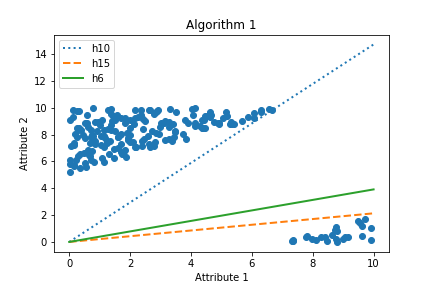
\includegraphics[scale=.5]{algorithm1}
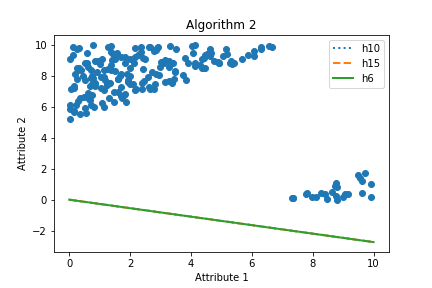
\includegraphics[scale=.5]{algorithm2}
\par
I have plotted only some of the hyperplanes with different $\alpha$ values for clarity. We can see from the scatter plots that algorithm 1 is more sensitive to $\alpha$ and that it allows the hyperplane to come closer to the examples. Algorithm 2 is less sensitive to $\alpha$, the hyperplane essentially overlap, and perhaps because of the margins and the few number of points in the bottom right the hyperplane lumps all points in the same classification. ...It also could be I made an error in the algorithm because this doesn't seem right...
\par
The table of weight vectors, shown in the jupyter notebook along with the code, also indicates the algorithm 2 is much less sensitive to $\alpha$.
\par
\subproblem{e} On the unsorted examples, the number of updates was  93  and the number of passes was  78.  On the sorted examples, The number of updates was  441  and the number of passes was  397.  Because the algorithm runs over the examples in order until a separating hyperplane is found, the sorted data groups together those which should not be separated so we have to cover more examples before finding an example that is classifed differently. While in the unsorted data, the algorithm gets to examples classified differently much earlier in looping over the examples. 

\end{document} 
